\documentclass{beamer}
\usetheme{Darmstadt}
\usecolortheme{beaver}
\useinnertheme{rectangles}
\setbeamertemplate{footline}[frame number]

\usepackage{lmodern}
\usepackage{natbib}
\usepackage{physics}
\usepackage{siunitx}
\usepackage{xcolor}
\usepackage{graphicx}
\usepackage{bbold}
\usepackage{mathtools}
\usepackage[compat=1.0.0]{tikz-feynman}
\usepackage{physics}

\definecolor{links}{HTML}{2A1B81}
\hypersetup{colorlinks,linkcolor=,urlcolor=links, citecolor=gray}

\usepackage{appendixnumberbeamer}
% \usepackage{hyperref}

% make bibliography entries smaller
\renewcommand\bibfont{\scriptsize}
% If you have more than one page of references, you want to tell beamer
% to put the continuation section label from the second slide onwards
\setbeamertemplate{frametitle continuation}[from second]
% Now get rid of all the colours
\setbeamercolor*{bibliography entry title}{fg=black}
\setbeamercolor*{bibliography entry author}{fg=black}
\setbeamercolor*{bibliography entry location}{fg=black}
\setbeamercolor*{bibliography entry note}{fg=black}
% and kill the abominable icon
\setbeamertemplate{bibliography item}{}

% kill tooltips
\setbeamertemplate{navigation symbols}{}

% \usepackage{beamerthemesplit} // Activate for custom appearance

\newcommand{\zcut}{z_\mathrm{cut}}

\title{Groomed jet mass}
\author{Kees Benkendorfer}
\institute{Reed College \\ Advisor: Andrew Larkoski}
% \institute{UM-CERN REU Final Presentation}
\date{17 March 2021 \\ Physics Seminar --- Senior Thesis Talks}
% \titlegraphic{\includegraphics[width=0.25\textwidth]{logos/reed_logo.jpg}}

\begin{document}

\begin{frame}[noframenumbering]
	\thispagestyle{empty}
	\titlepage
\end{frame}

\section[Outline]{}
\frame{\tableofcontents}


\section{Searching for new physics}
	\begin{frame}
		\frametitle{The Standard Model}
		\begin{center}
			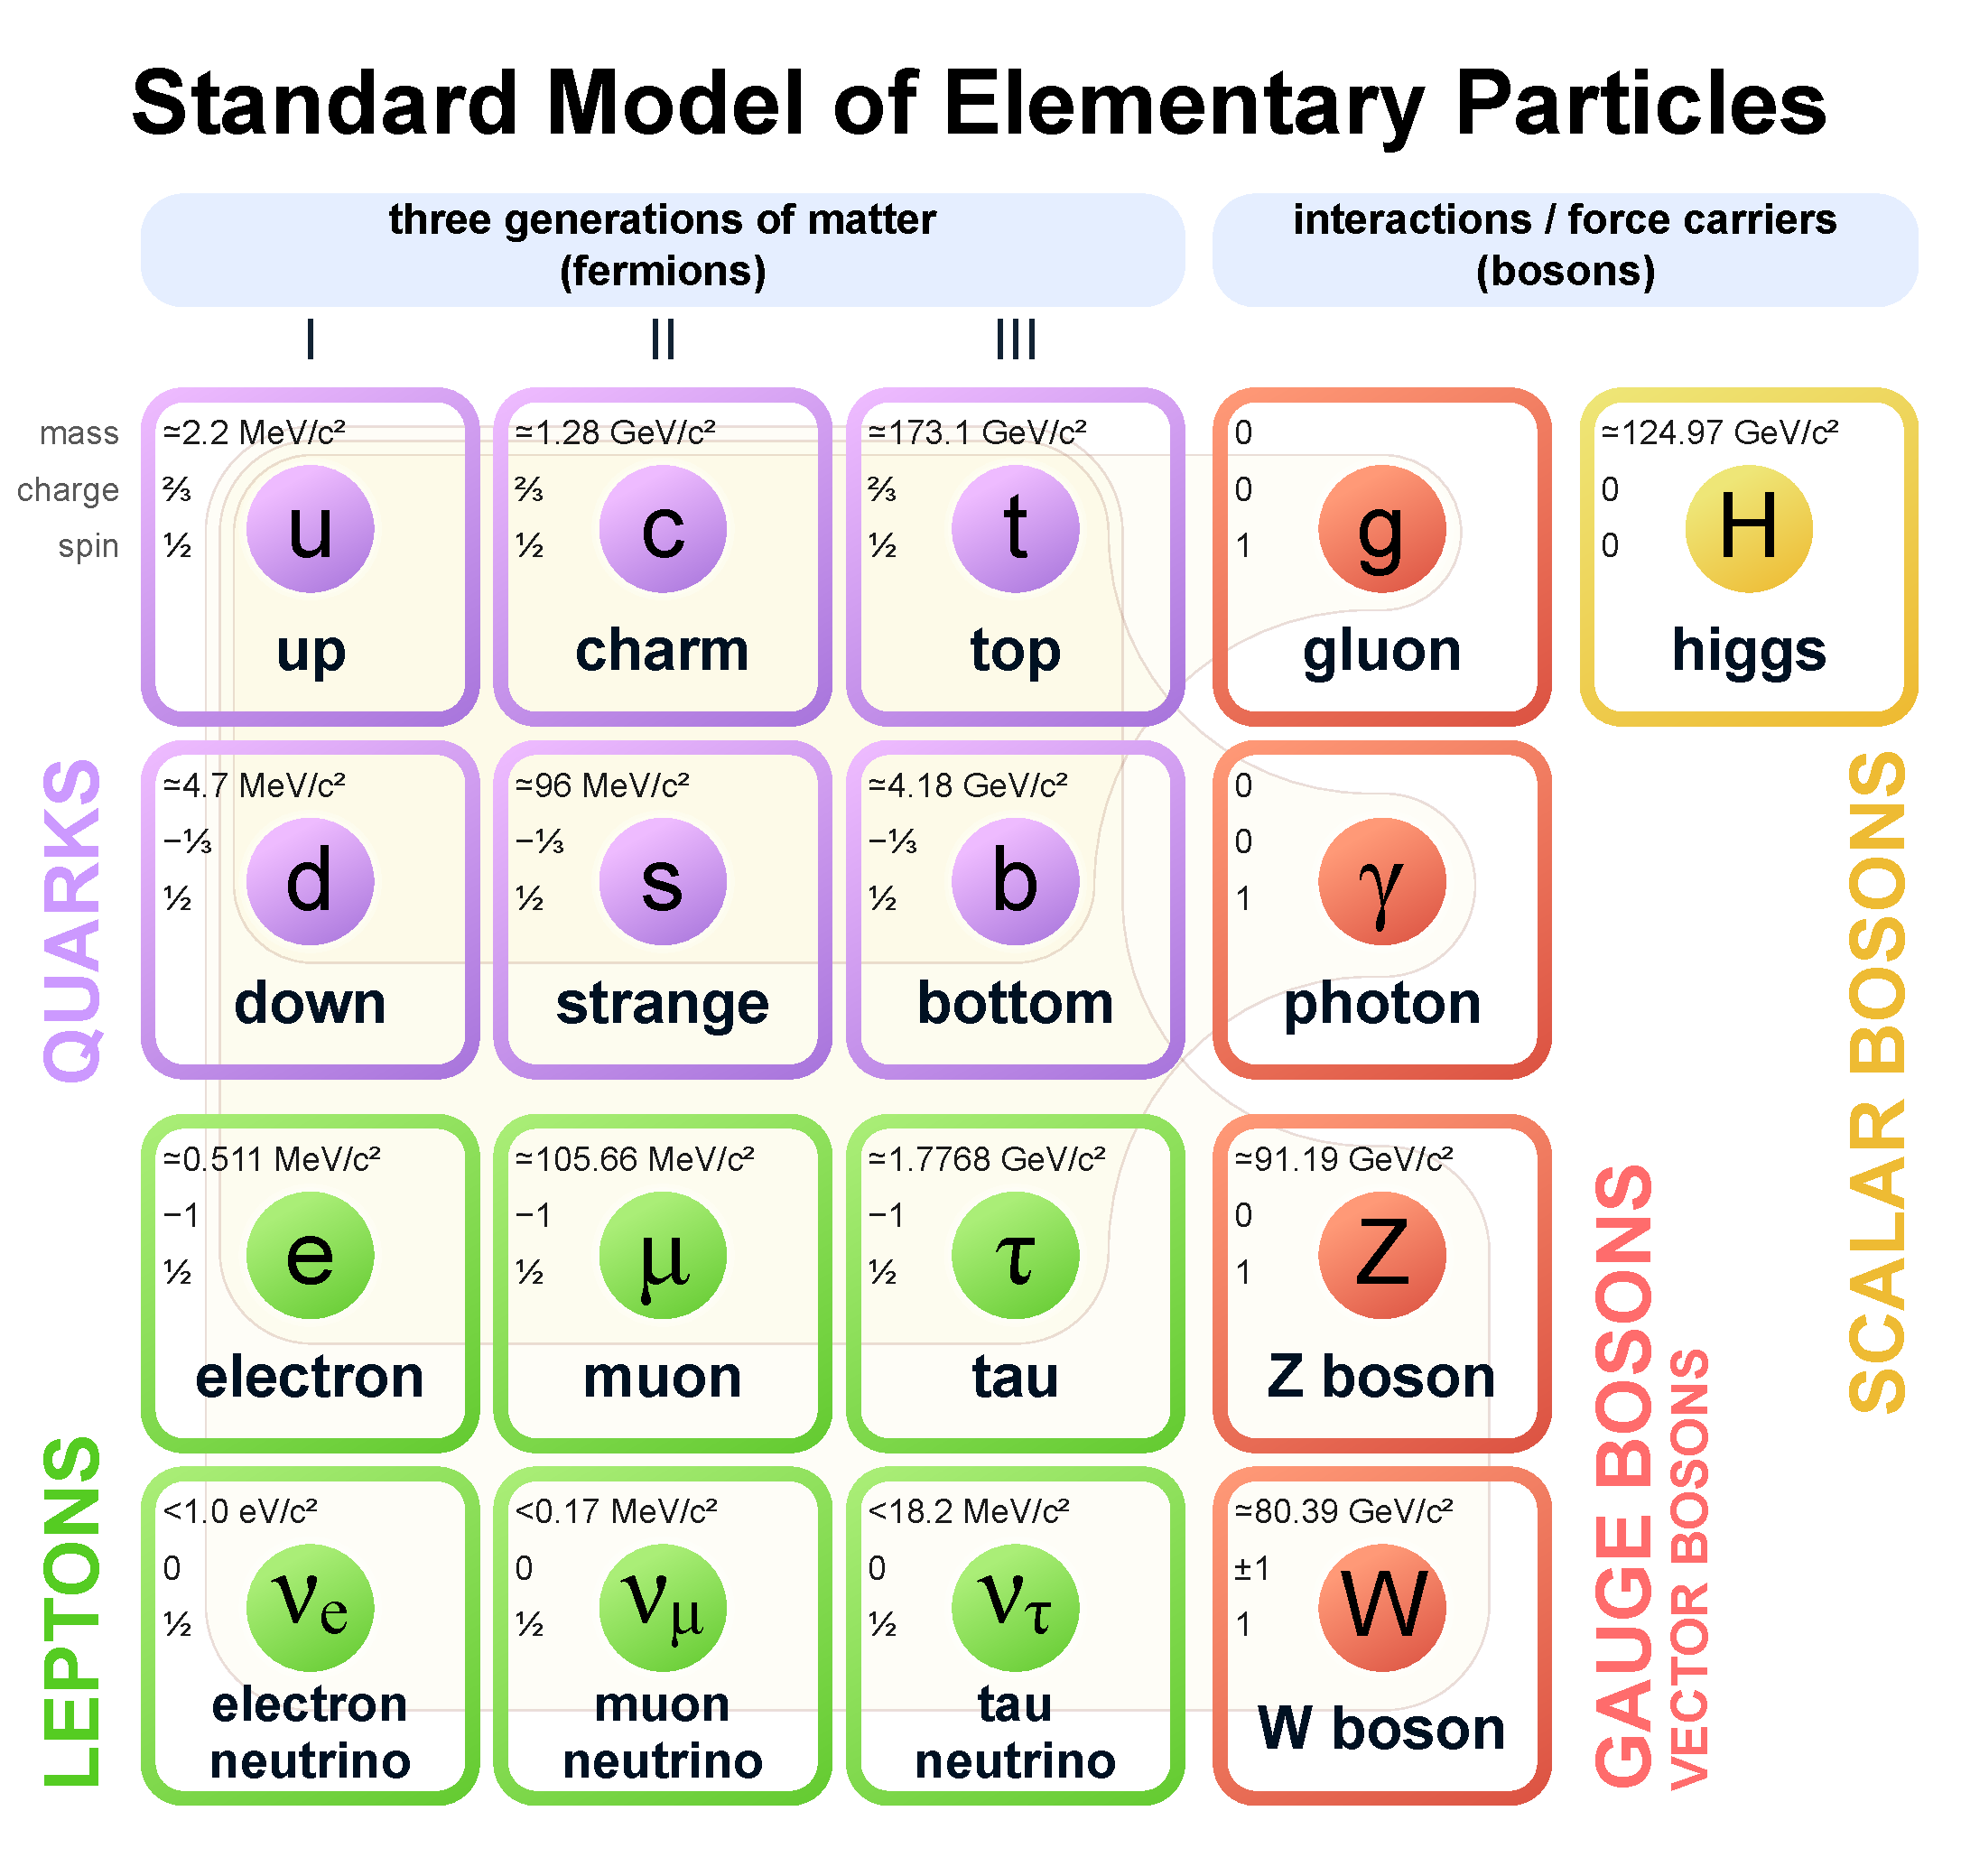
\includegraphics[width=0.6\textwidth]{figures/Standard_Model_of_Elementary_Particles.pdf}
		\end{center}
	\end{frame}

	\begin{frame}
		\frametitle{Searching for new physics}

		\begin{columns}
		\column{0.5\textwidth}
			\begin{itemize}
				\item Direct particle searches
				\begin{itemize}
					\item Resonance searches

					\item Low-background detectors
				\end{itemize}

				\item<2-> \textbf{Precisions measurements}
			\end{itemize}

			\vspace{0.5cm}

			\onslide<2->{
			\begin{figure}
				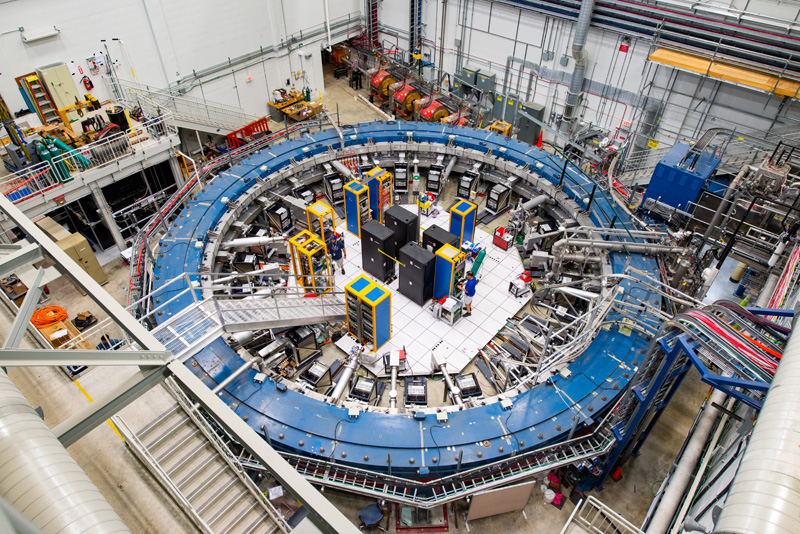
\includegraphics[width=0.75\columnwidth]{figures/muon_g_2.jpeg}
				\caption{Muon $g-2$ experiment, from \url{https://vms.fnal.gov/gallery/view?id=41}}
			\end{figure}
			}

		\column{0.5\textwidth}
			\begin{figure}
				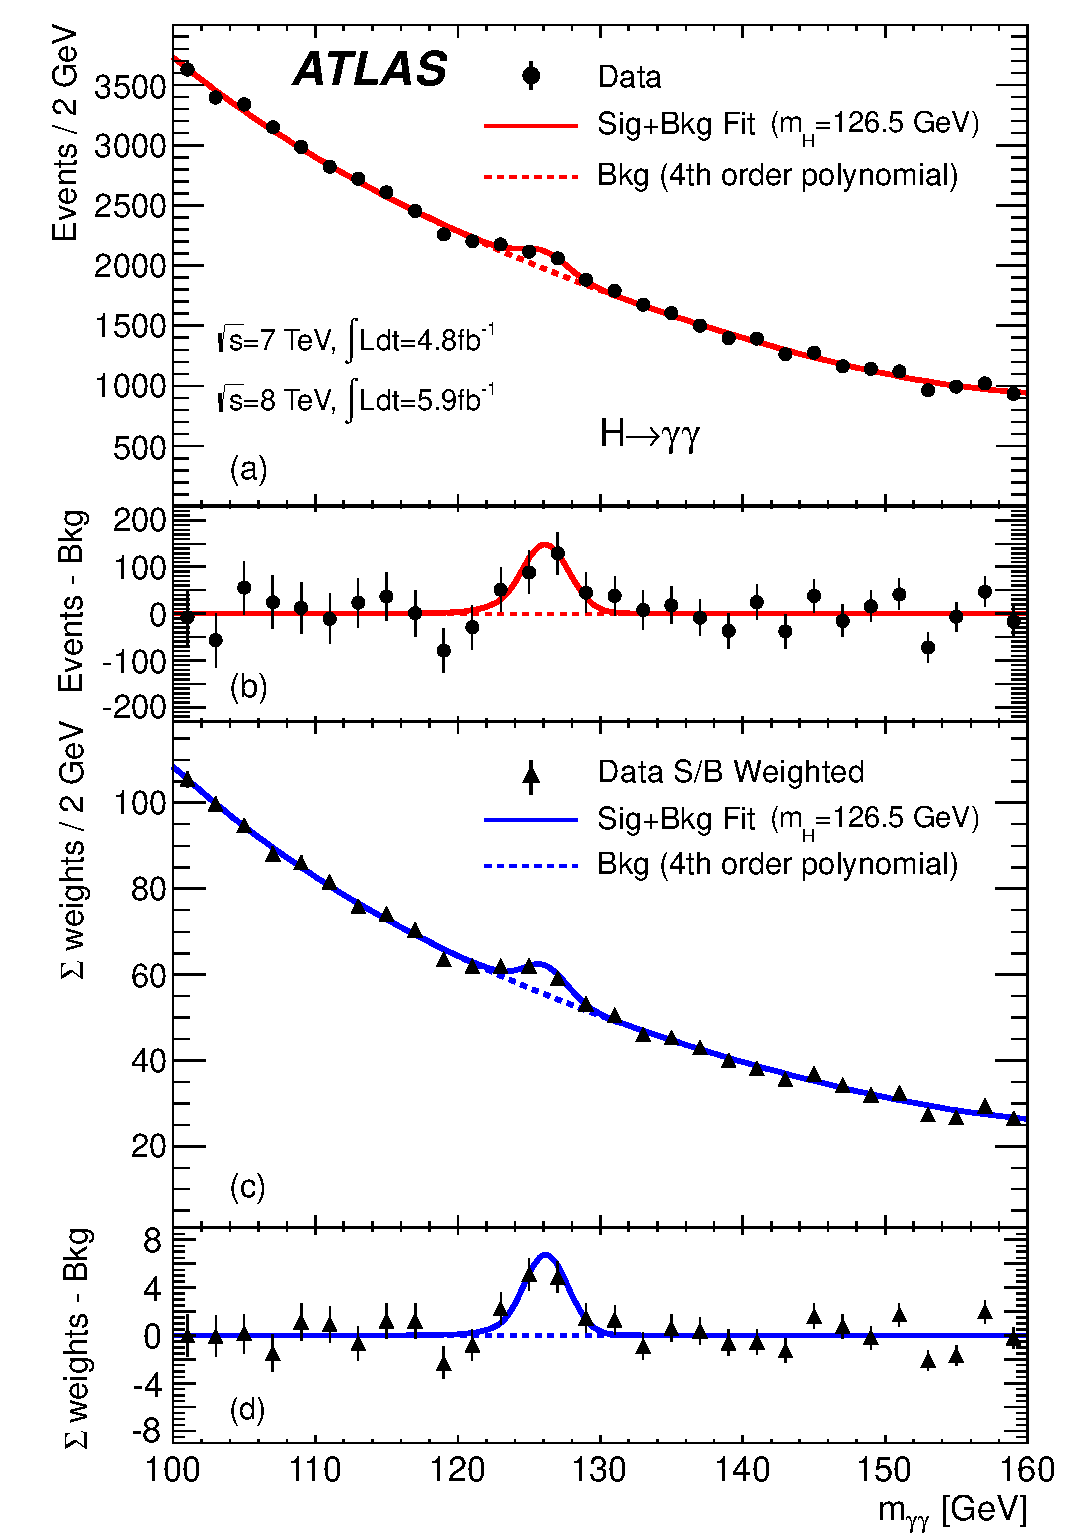
\includegraphics[width=0.75\columnwidth]{figures/higgs_discovery.pdf}
				\caption{Higgs boson discovery by ATLAS, from \cite{atlas_collaboration_observation_2012}}
			\end{figure}
		\end{columns}
	\end{frame}


\section{Quantum chromodynamics}
	\begin{frame}
		\frametitle{Quantum chromodynamics (QCD)}

		\begin{columns}
		\column{0.5\textwidth}
			\begin{itemize}
				\item Theory of the strong force

				\item Like the electric force
				\begin{itemize}
					\item Particles have \textbf{color charge}

					\item QCD version of photon is the \textbf{gluon}
				\end{itemize}

				\item Interesting nonlinear dynamics:
				\begin{itemize}
					\item Self-coupling

					\item Scale-invariance

					\item Confinement
				\end{itemize}
			\end{itemize}

		\column{0.5\textwidth}
		\begin{figure}
			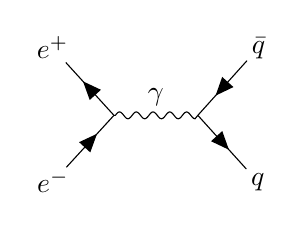
\begin{tikzpicture}
			\begin{feynman}[scale=0.7]
				\diagram [horizontal=a to b] {
	  				i1 [particle=\(e^{-}\)] -- [fermion] a -- [fermion] i2 [particle=\(e^{+}\)],
	  				a -- [photon, edge label=\(\gamma\)] b,
	  				f1 [particle=\(\bar q\)] -- [fermion] b -- [fermion] f2 [particle=\(q\)],
				};
			\end{feynman}
			\end{tikzpicture}

			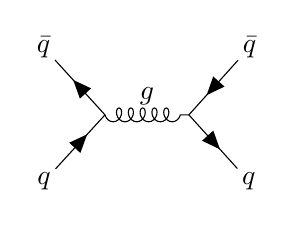
\begin{tikzpicture}
			\begin{feynman}[scale=0.7]
				\diagram [horizontal=a to b] {
	  				i1 [particle=\(q\)] -- [fermion] a -- [fermion] i2 [particle=\(\bar{q}\)],
	  				a -- [gluon, edge label=\(g\)] b,
	  				f1 [particle=\(\bar q\)] -- [fermion] b -- [fermion] f2 [particle=\(q\)],
				};
			\end{feynman}
			\end{tikzpicture}

			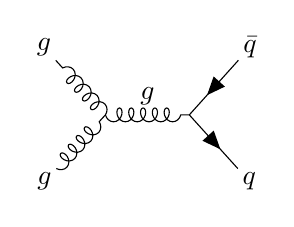
\begin{tikzpicture}
			\begin{feynman}[scale=0.7]
				\diagram [horizontal=a to b] {
	  				i1 [particle=\(g\)] -- [gluon] a -- [gluon] i2 [particle=\(g\)],
	  				a -- [gluon, edge label=\(g\)] b,
	  				f1 [particle=\(\bar q\)] -- [fermion] b -- [fermion] f2 [particle=\(q\)],
				};
			\end{feynman}
			\end{tikzpicture}
		\end{figure}
		\end{columns}
	\end{frame}

	\begin{frame}
		\frametitle{Jets}

		\begin{itemize}
			\item High-energy quarks and gluons $\to$ collimated sprays of hadronic particles in detector

			\item These sprays are called \textbf{jets}

			\item Rich substructure can be used to probe Standard Model
			\begin{itemize}
				\item \textbf{Jet mass}, number of particles, number of `prongs', etc

				\item Would like, e.g., to measure strong coupling constant $\alpha_s$
			\end{itemize}
		\end{itemize}
	\end{frame}

	\begin{frame}
		\frametitle{Jet example}
		\begin{figure}
			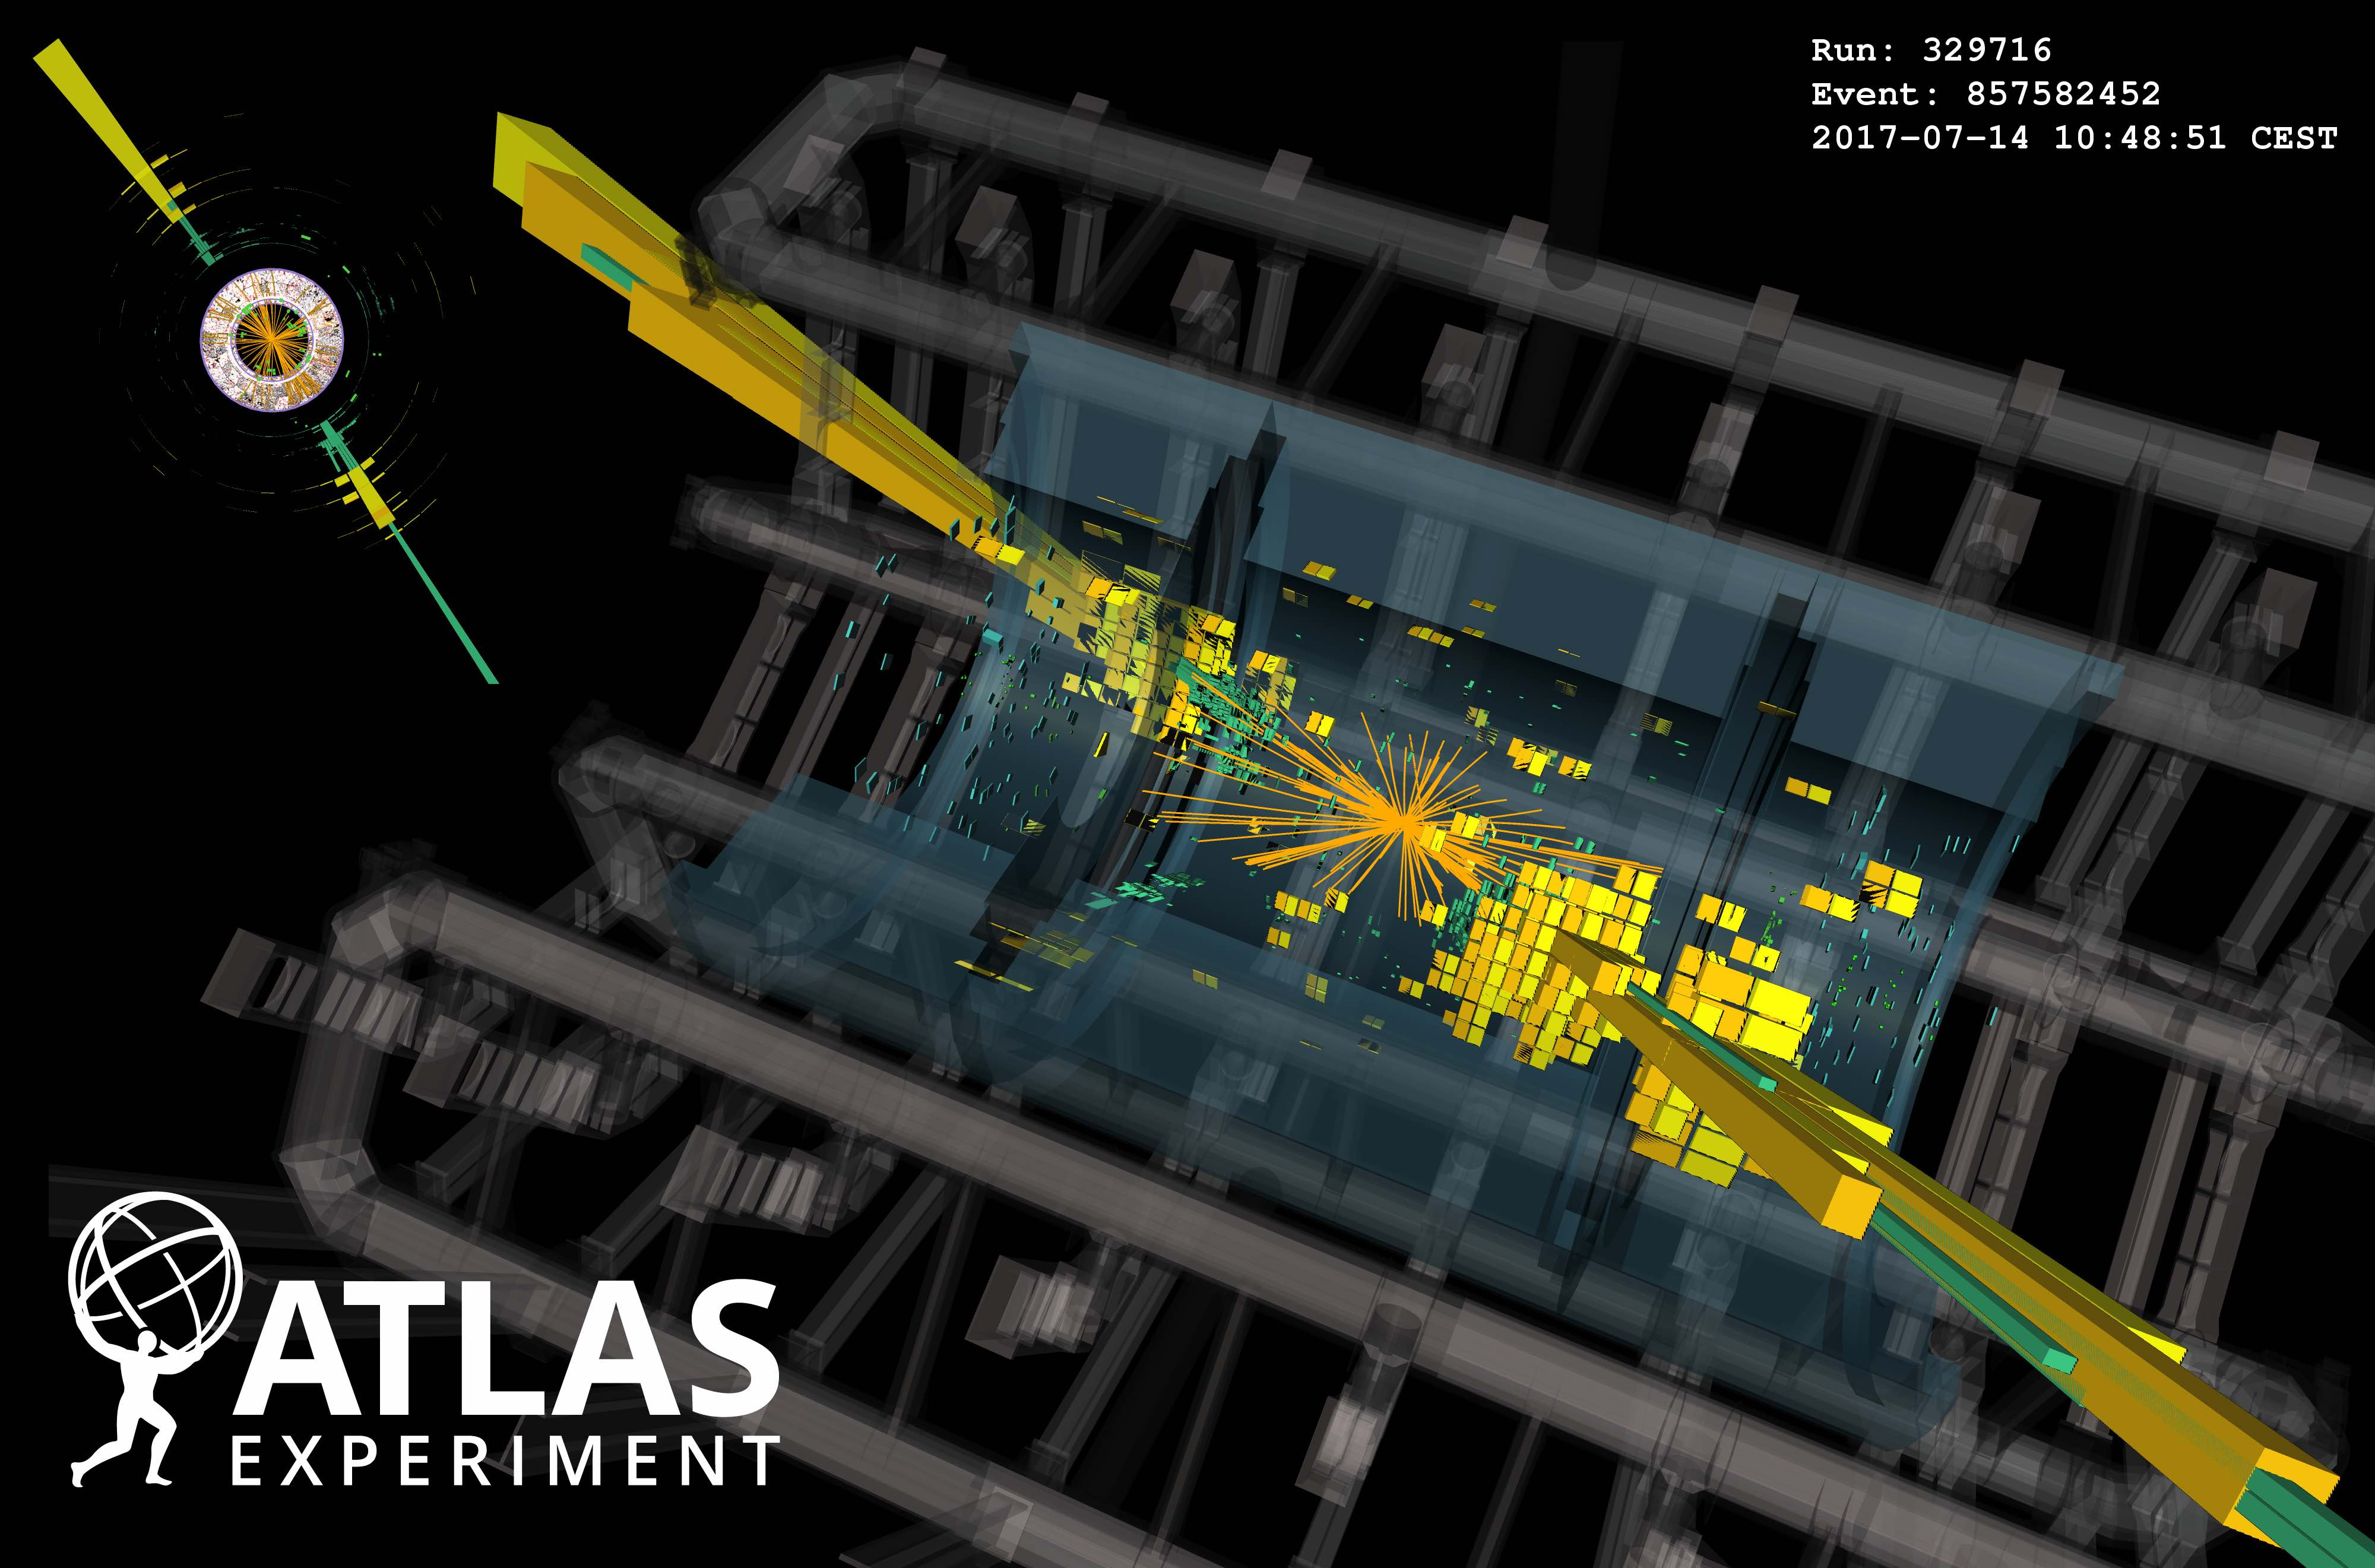
\includegraphics[width=0.8\columnwidth]{figures/DijetHighMass9.3TeV-VP1-nocone_small.jpg}

			\caption{Dijet (two-jet) event captured by ATLAS in 2017. From \url{https://twiki.cern.ch/twiki/bin/view/AtlasPublic/EventDisplayRun2Physics}}
		\end{figure}
	\end{frame}


\section{Jet grooming}
	\begin{frame}
		\frametitle{Experimental problems with jets}

		\begin{itemize}
			\item Other events in the detector might contaminate measurements
		\end{itemize}

		\vfill

		\begin{figure}
			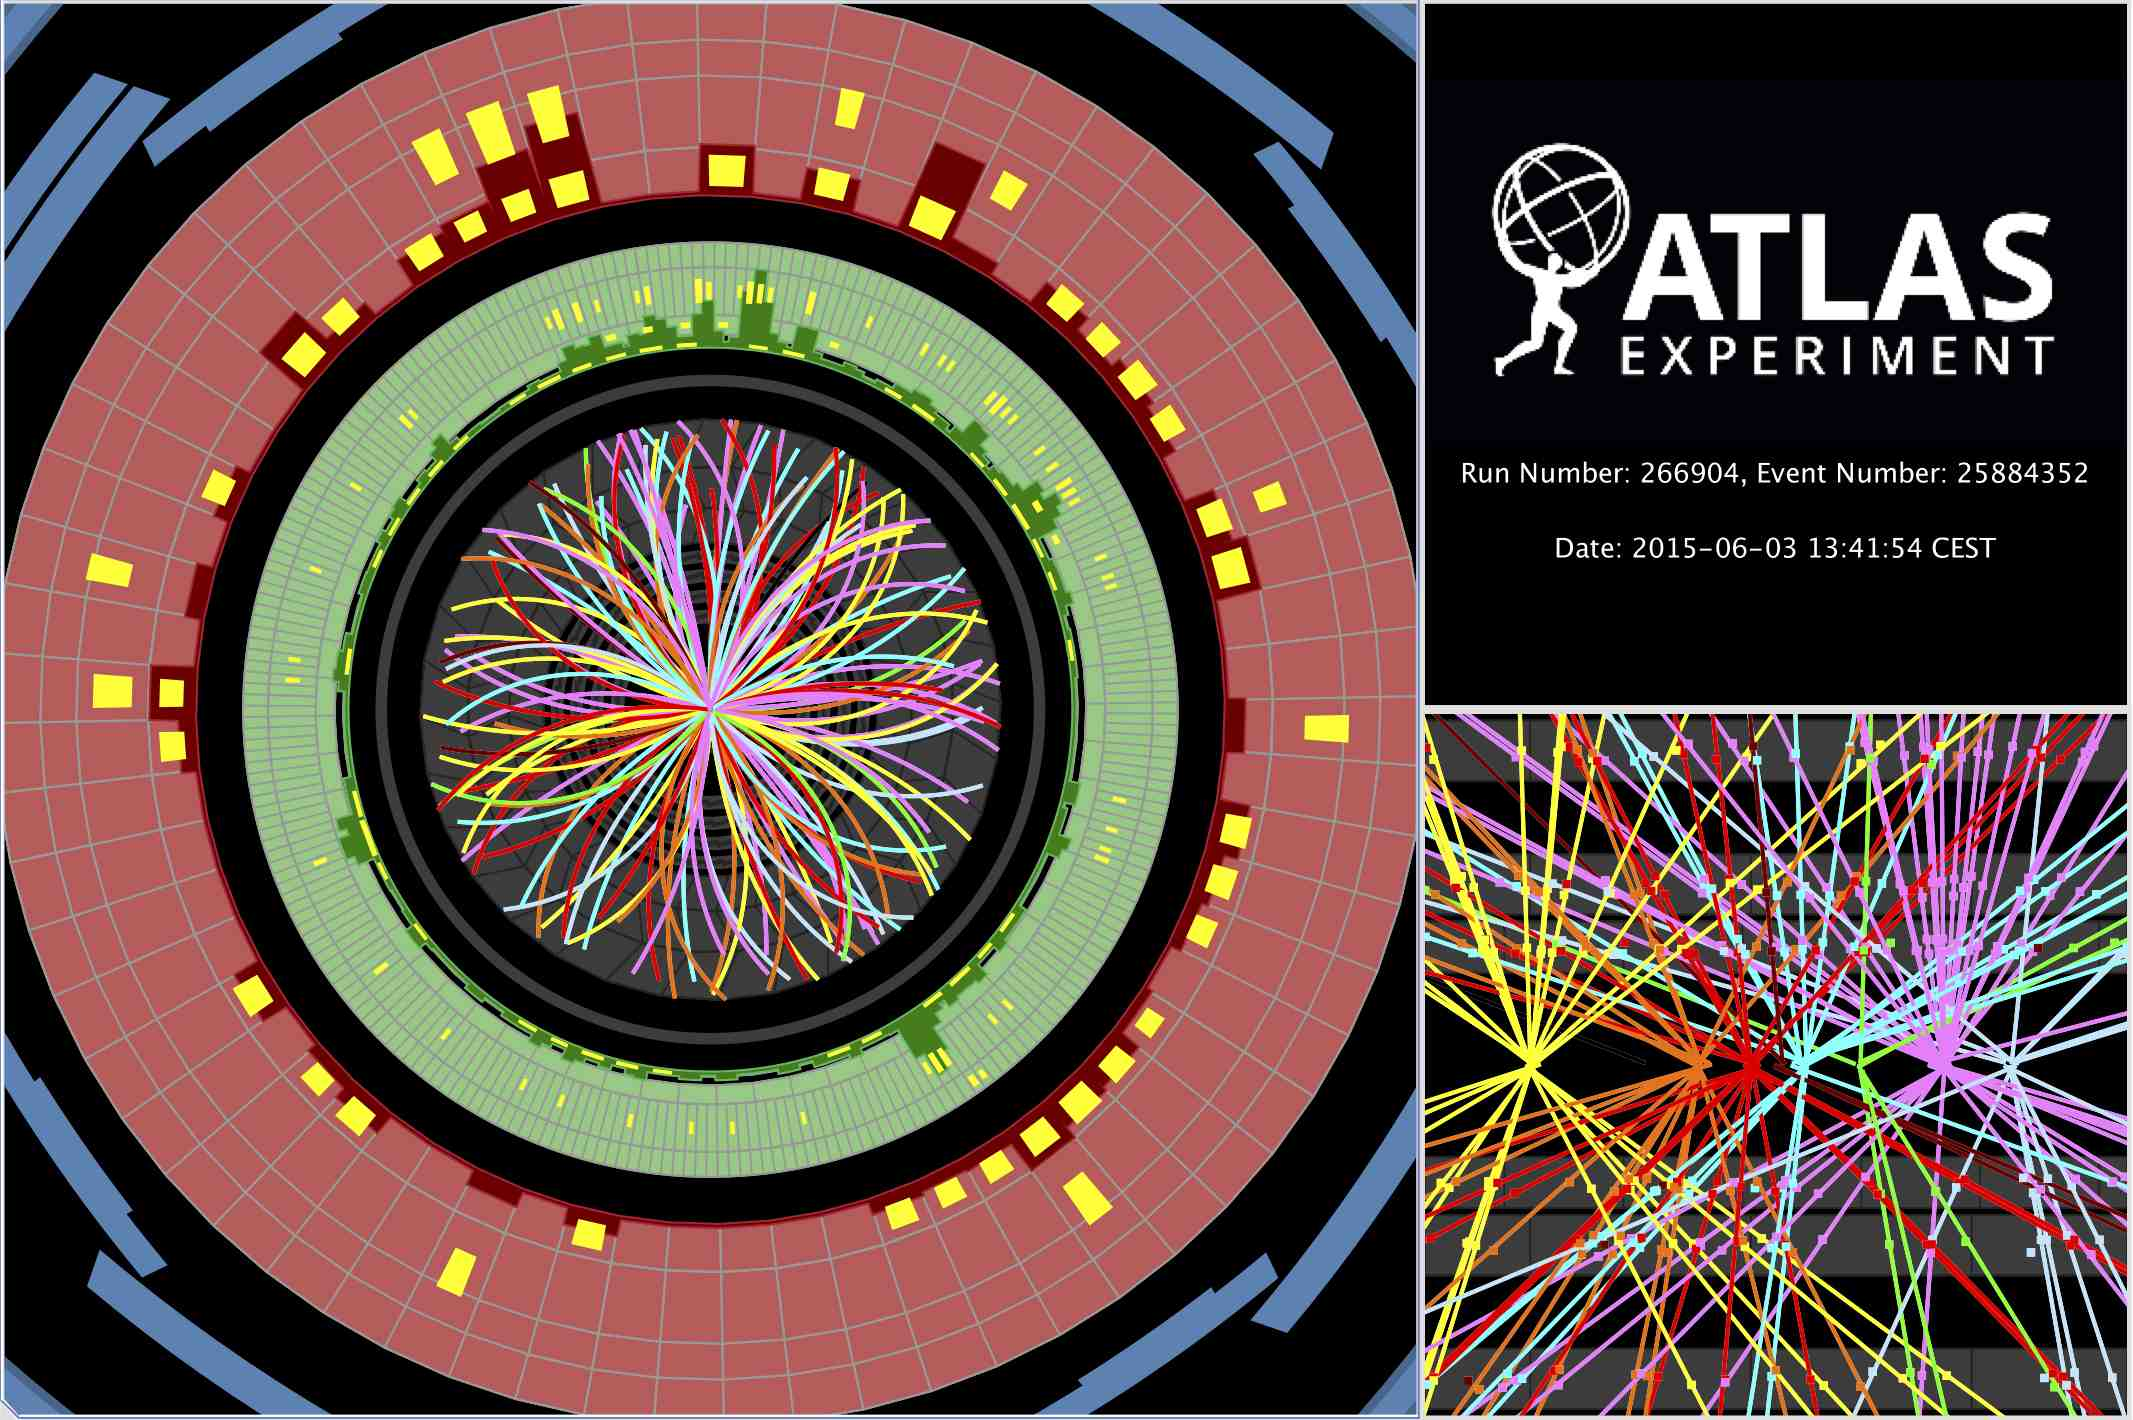
\includegraphics[width=0.7\textwidth]{figures/atlas_pile_up.jpeg}
			\caption{Collision event with significant `pile-up' at ATLAS in 2015. From \url{https://twiki.cern.ch/twiki/bin/view/AtlasPublic/EventDisplayRun2Collisions}}
		\end{figure}
	\end{frame}

	\begin{frame}
		\frametitle{Theoretical problems with jets}

		\begin{itemize}
			\item Very difficult to characterize corrections to jet substructure from out-of-jet radiation
			\begin{itemize}
				\item Hadronization is complicated
			\end{itemize}

			\item Separation between energy scale of jet and energy scale of background causes problems
			\begin{itemize}
				\item Produces large so-called `non-global logarithms' \cite{kardos_groomed_2020}
			\end{itemize}

			\item If we have two scales $\omega_1$ and $\omega_2$ with $\omega_1 \ll \omega_2$, might find large terms like
			\begin{equation*}
				\log \frac{\omega_1}{\omega_2}
			\end{equation*}
		\end{itemize}
	\end{frame}

	\begin{frame}
		\frametitle{Solution: jet grooming}

		\begin{itemize}
			\item \textbf{Idea:} clear away low-energy (\textbf{soft}) radiation below some threshold $\zcut$
			\begin{itemize}
				\item We lose some jet events, but mostly background events
			\end{itemize}
		\end{itemize}

		\vspace{1cm}

		\begin{figure}
			\raisebox{-.5\height}{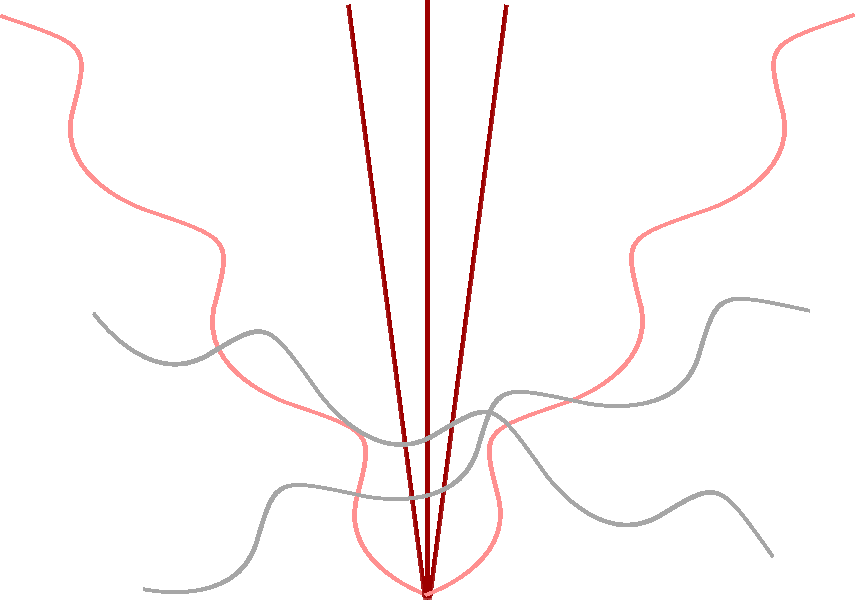
\includegraphics[width=0.45\columnwidth]{figures/jet_grooming.pdf}}
		\end{figure}
	\end{frame}

	\begin{frame}
		\frametitle{Solution: jet grooming}

		\begin{itemize}
			\item \textbf{Idea:} clear away low-energy (\textbf{soft}) radiation below some threshold $\zcut$
			\begin{itemize}
				\item We lose some jet events, but mostly background events
			\end{itemize}
		\end{itemize}

		\vspace{1cm}

		\begin{figure}
			\raisebox{-.5\height}{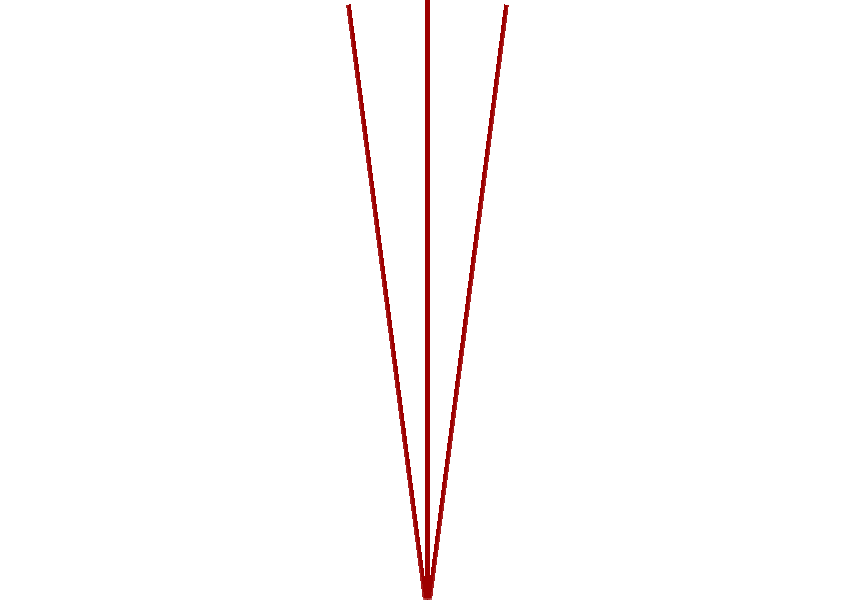
\includegraphics[width=0.45\columnwidth]{figures/jet_grooming_post_groom.pdf}}
		\end{figure}
	\end{frame}

\section{Jet mass}
	\begin{frame}
		\frametitle{Observable of choice}
		
		\begin{itemize}
			\item We want to look at $e^+ e^- \to \text{hemisphere jets}$ events

			\item Measure the mass of the heavier hemisphere
		\end{itemize}
		\begin{figure}
			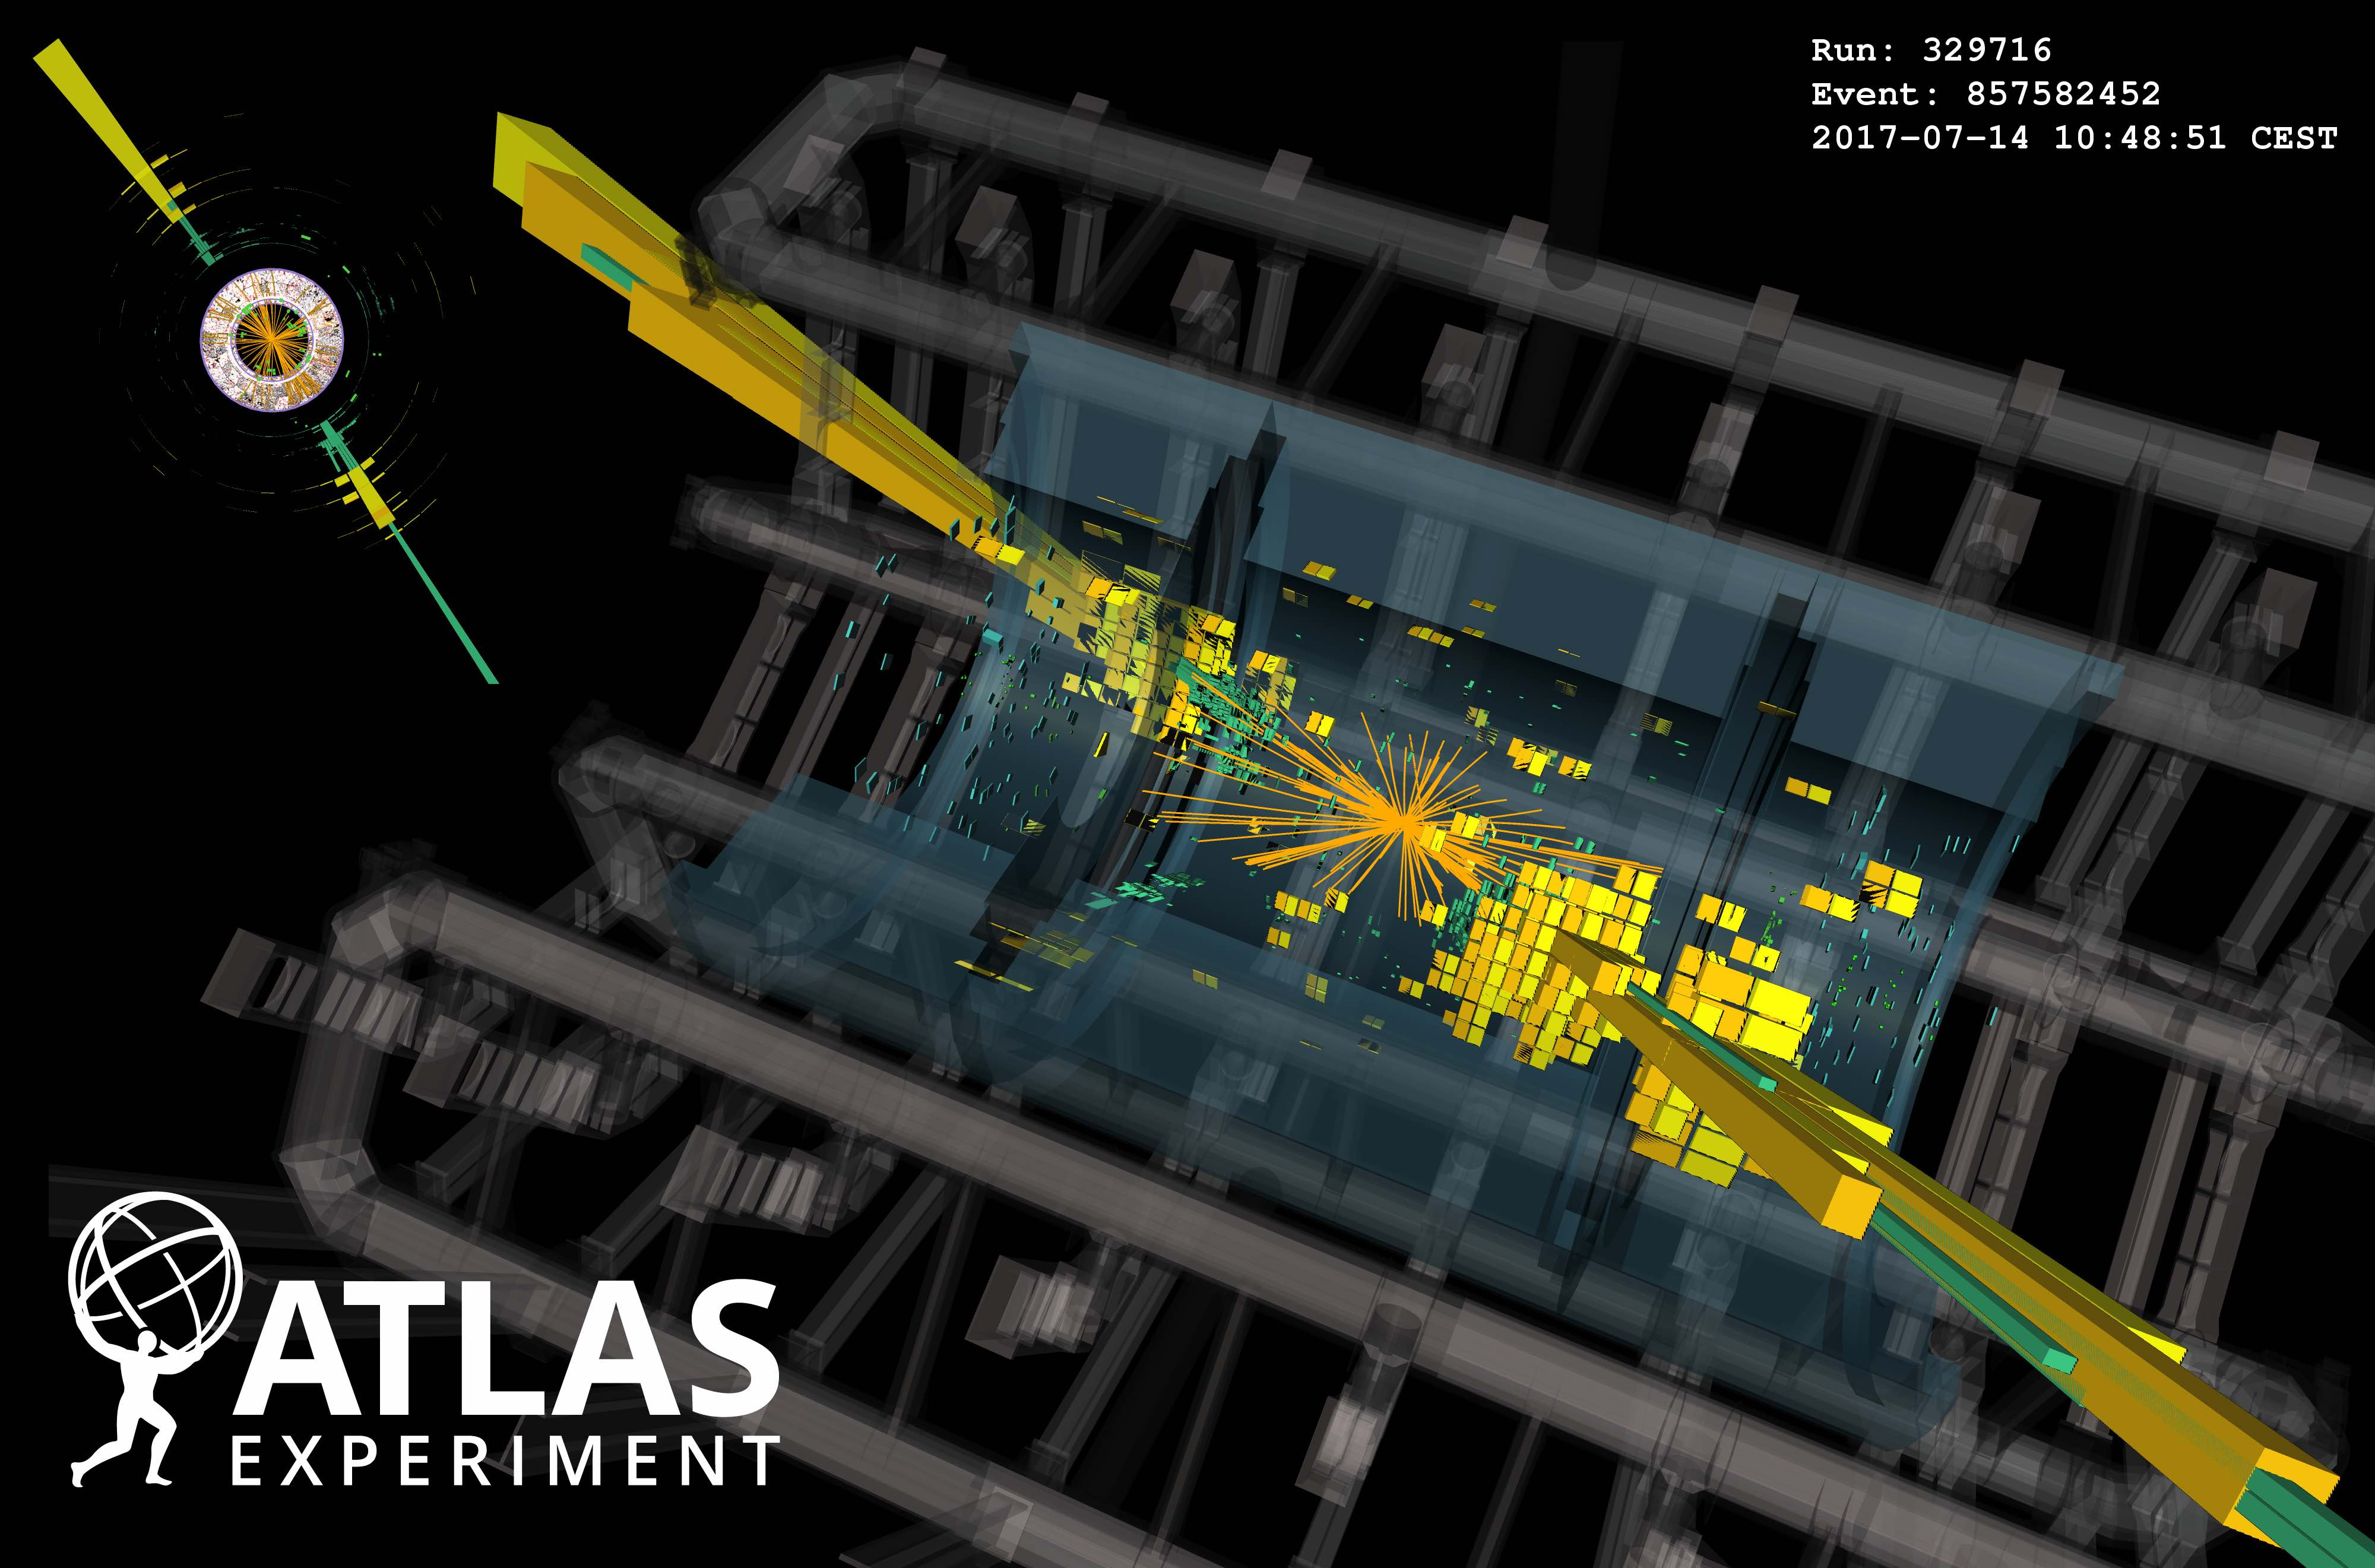
\includegraphics[width=0.75\textwidth]{figures/DijetHighMass9.3TeV-VP1-nocone_small.jpg}
		\end{figure}

		\onslide<2->{%
			\tikz[overlay,remember picture]
			\draw[thick, red] (2.5, 3) -- (6, 3) -- (6, 5.75) -- (2.5, 5.75) -- cycle;
		}

		\onslide<2->{%
			\tikz[overlay,remember picture]
			\node[fill=black,text=white] at ([xshift=-5cm,yshift=-1cm]current page.center){measure mass};
			\tikz[overlay, remember picture]
			\draw[thick, red, ->] (1.5, 4) -- (2.25, 4.5);
		}

		\onslide<2->{%
			\tikz[overlay,remember picture]
			\draw[thick, red] (9.5, 1.5) -- (6, 1.5) -- (6, 5) -- (9.5, 5) -- cycle;
		}

		\onslide<2->{%
			\tikz[overlay,remember picture]
			\node[fill=black,text=white] at ([xshift=5cm,yshift=-1cm]current page.center){measure mass};
			\tikz[overlay, remember picture]
			\draw[thick, red, ->] (10.5, 4.25) -- (9.5, 3.5);
		}
	\end{frame}

	\begin{frame}
		\frametitle{Recent experimental measurement}
		\begin{figure}
			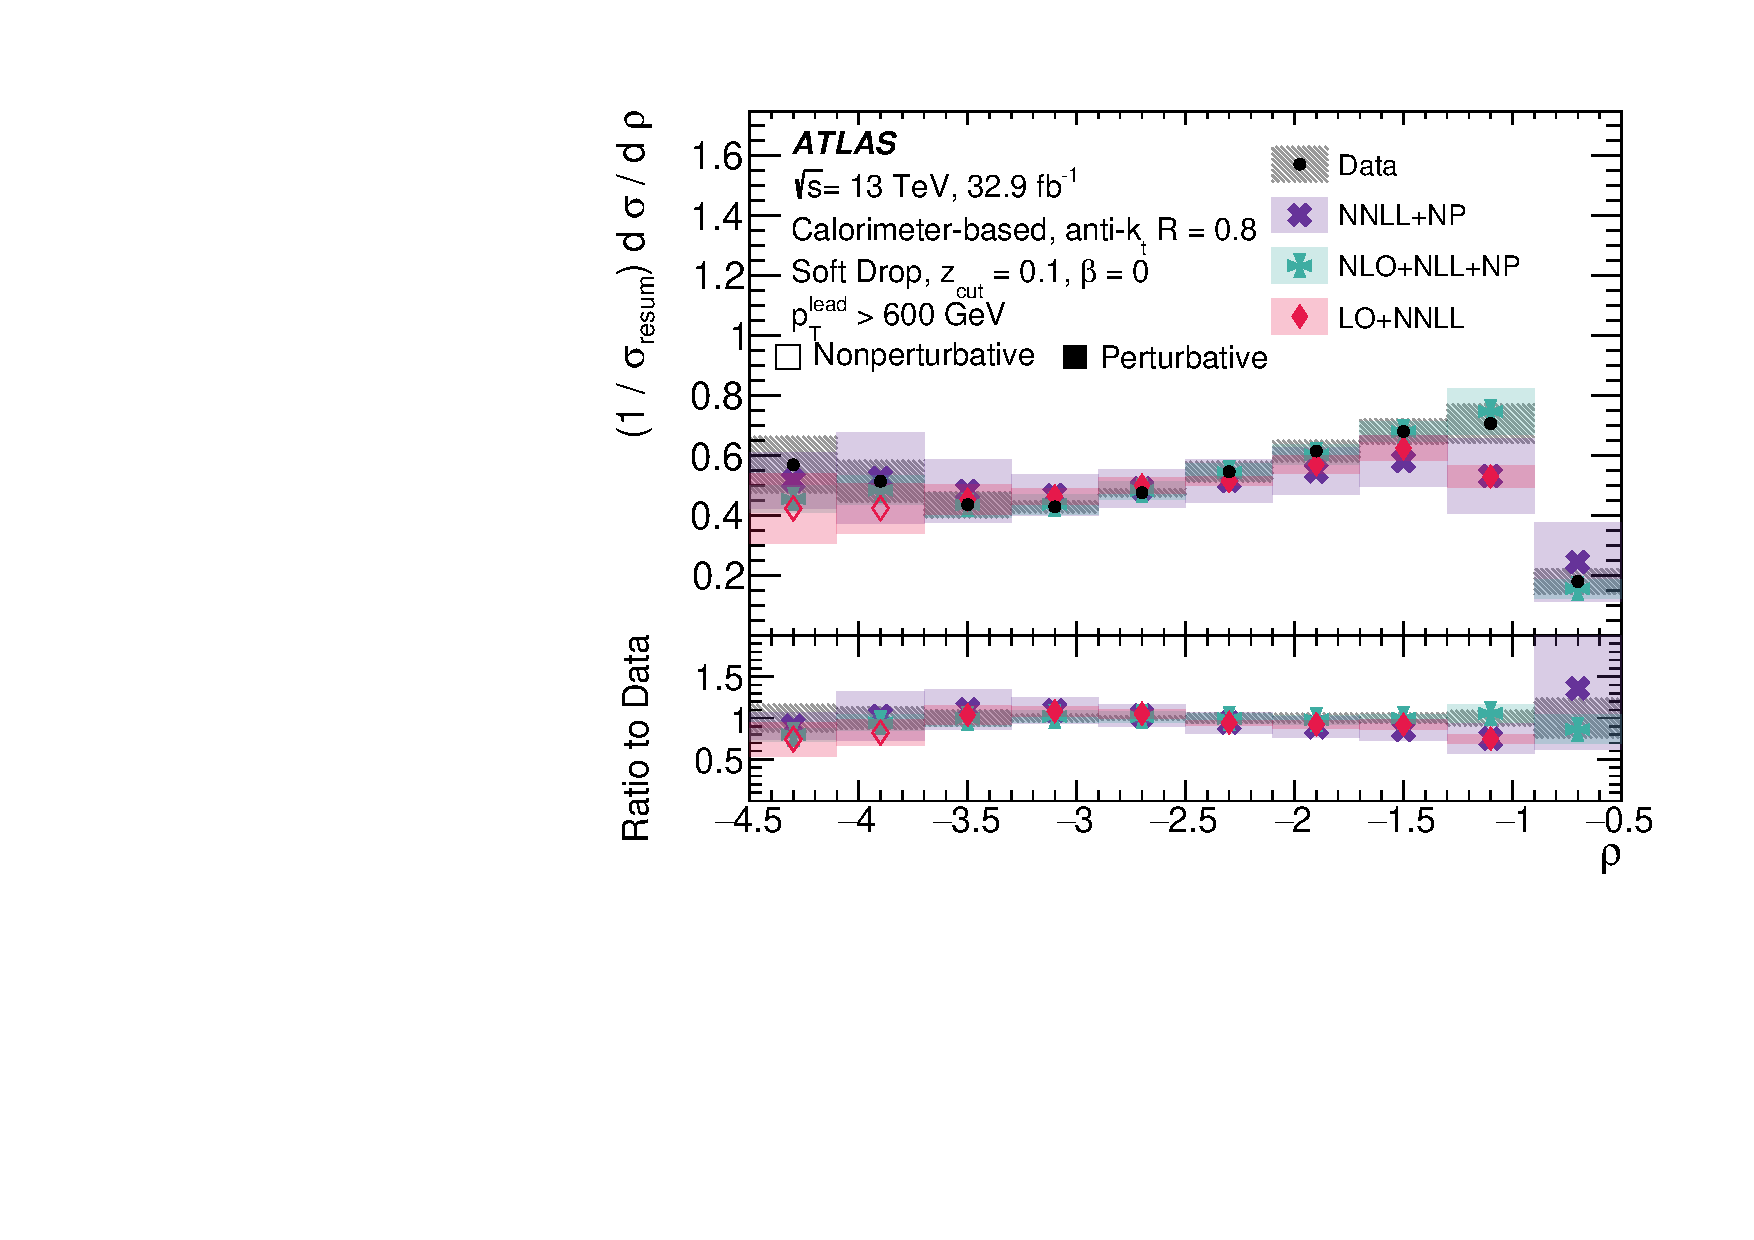
\includegraphics[width=0.75\textwidth]{figures/atlas_mass_measurement.pdf}

			\caption{(Dimensionless) groomed jet mass measurement by ATLAS in 2020. (Note: this is not heavy hemisphere mass). From \cite{atlas_collaboration_measurement_2020}}
		\end{figure}
	\end{frame}

	\begin{frame}
		\frametitle{Recent theoretical results}

		\begin{figure}
			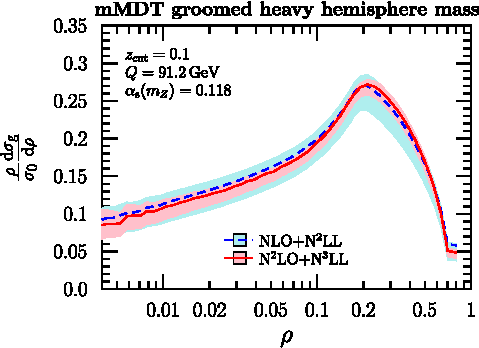
\includegraphics[width=0.75\textwidth]{figures/kardos_et_al_groomed_hemisphere_mass.pdf}

			\caption{Most precise theoretical calculation of groomed jet mass to date by Kardos, Larkoski, and Tr\`ocs\`anyi. From \cite{kardos_groomed_2020}}
		\end{figure}

		\onslide<2->{%
			\tikz[overlay,remember picture]
			\node at ([xshift=-4.5cm,yshift=2cm]current page.center){$\rho \ll \zcut \ll 1$};
			\tikz[overlay, remember picture]
			\draw[thick, red, ->] (1.5, 6.75) -- (4, 4.75);
		}
		\onslide<2->{%
			\tikz[overlay,remember picture]
			\node at ([xshift=5cm,yshift=1cm]current page.center){$\rho \sim 1$};
			\tikz[overlay, remember picture]
			\draw[thick, red, ->] (9.75, 5.75) -- (8.25, 4.75);
		}
		\onslide<2->{%
			\tikz[overlay,remember picture]
			\draw[thick, red] (6, 5.5) -- (7.5, 5.5) -- (7.5, 7) -- (6, 7) -- cycle;
		}
		\onslide<2->{%
			\tikz[overlay,remember picture]
			\node at ([xshift=5.25cm,yshift=2cm]current page.center){$\rho \sim \zcut \ll 1$};
			\tikz[overlay, remember picture]
			\draw[thick, red, ->] (8.35, 6.75) -- (7.25, 6.25);
		}
	\end{frame}


\section{My thesis}
	\begin{frame}
		\frametitle{My thesis: calculating the cusp region}

		\begin{itemize}
			\item Calculations in QCD often must be done as a Taylor expansion

			\item \textbf{Goal:} perform an `all-orders' calculation in the cusp region
			\begin{itemize}
				\item Overall expression which describes all terms of the expansion in terms of an integral

				\item Accuracy can be increased by calculating higher-order terms of integrand
			\end{itemize}

			\item Terms take the form \cite{frye_factorization_2016}
			\begin{equation*}
			\begin{aligned}
				F(\mu) = F(\mu_0) \exp\Bigg[2\int_{\alpha_s(\mu_0)}^{\alpha_s(\mu)} &\frac{d\alpha}{\beta(\alpha)}\Gamma_F(\alpha)\int_{\alpha_s(\mu_0)}^\alpha \frac{d\alpha'}{\beta(\alpha')} \\
				&+ \int_{\alpha_s(\mu_0)}^{\alpha_s(\mu)} \frac{d\alpha}{\beta(\alpha)}\gamma_F(\alpha) \\
				&+ \log \frac{\mu_0^2}{\mu_1^2}\int_{\alpha_s(\mu_0)}^{\alpha_s(\mu)} \frac{d\alpha}{\beta(\alpha)}\Gamma_F(\alpha) \Bigg]
			\end{aligned}
			\end{equation*}
		\end{itemize}
	\end{frame}

	\begin{frame}
		\frametitle{Day-to-day work}
		\begin{itemize}
			\item Many weird, big integrals

			\item Lots of fun mathematical trickery involved for the curious

			\item Working in $4 - 2\epsilon$ dimensions so that we can calculate divergent integrals

			\begin{equation*}
			\begin{aligned}
				\int d^4p \,f(p) &= \infty \\
				\int d^{4-2\epsilon}p\, f(p) &< \infty
			\end{aligned}
			\end{equation*}

			\item And more!
		\end{itemize}
	\end{frame}


\section*{}
    \begin{frame}[allowframebreaks]
        \frametitle{References}
        \bibliographystyle{unsrt}
        %\bibliographystyle{amsalpha}
        \bibliography{jet_substructure}
    \end{frame}

\end{document}
